\documentclass{standalone}
\usepackage{fontspec}
\setmainfont[Scale=1.5]{Tex Gyre Heros}

\usepackage[dvipsnames]{xcolor}
\usepackage{tikz}

\tikzset{score rectangle/.style={draw, inner sep=0pt, minimum height=52mm, minimum width=27mm}}
\tikzset{score circle/.style={draw, ultra thick, inner sep=0pt, circle, minimum width=20mm}}



\begin{document}
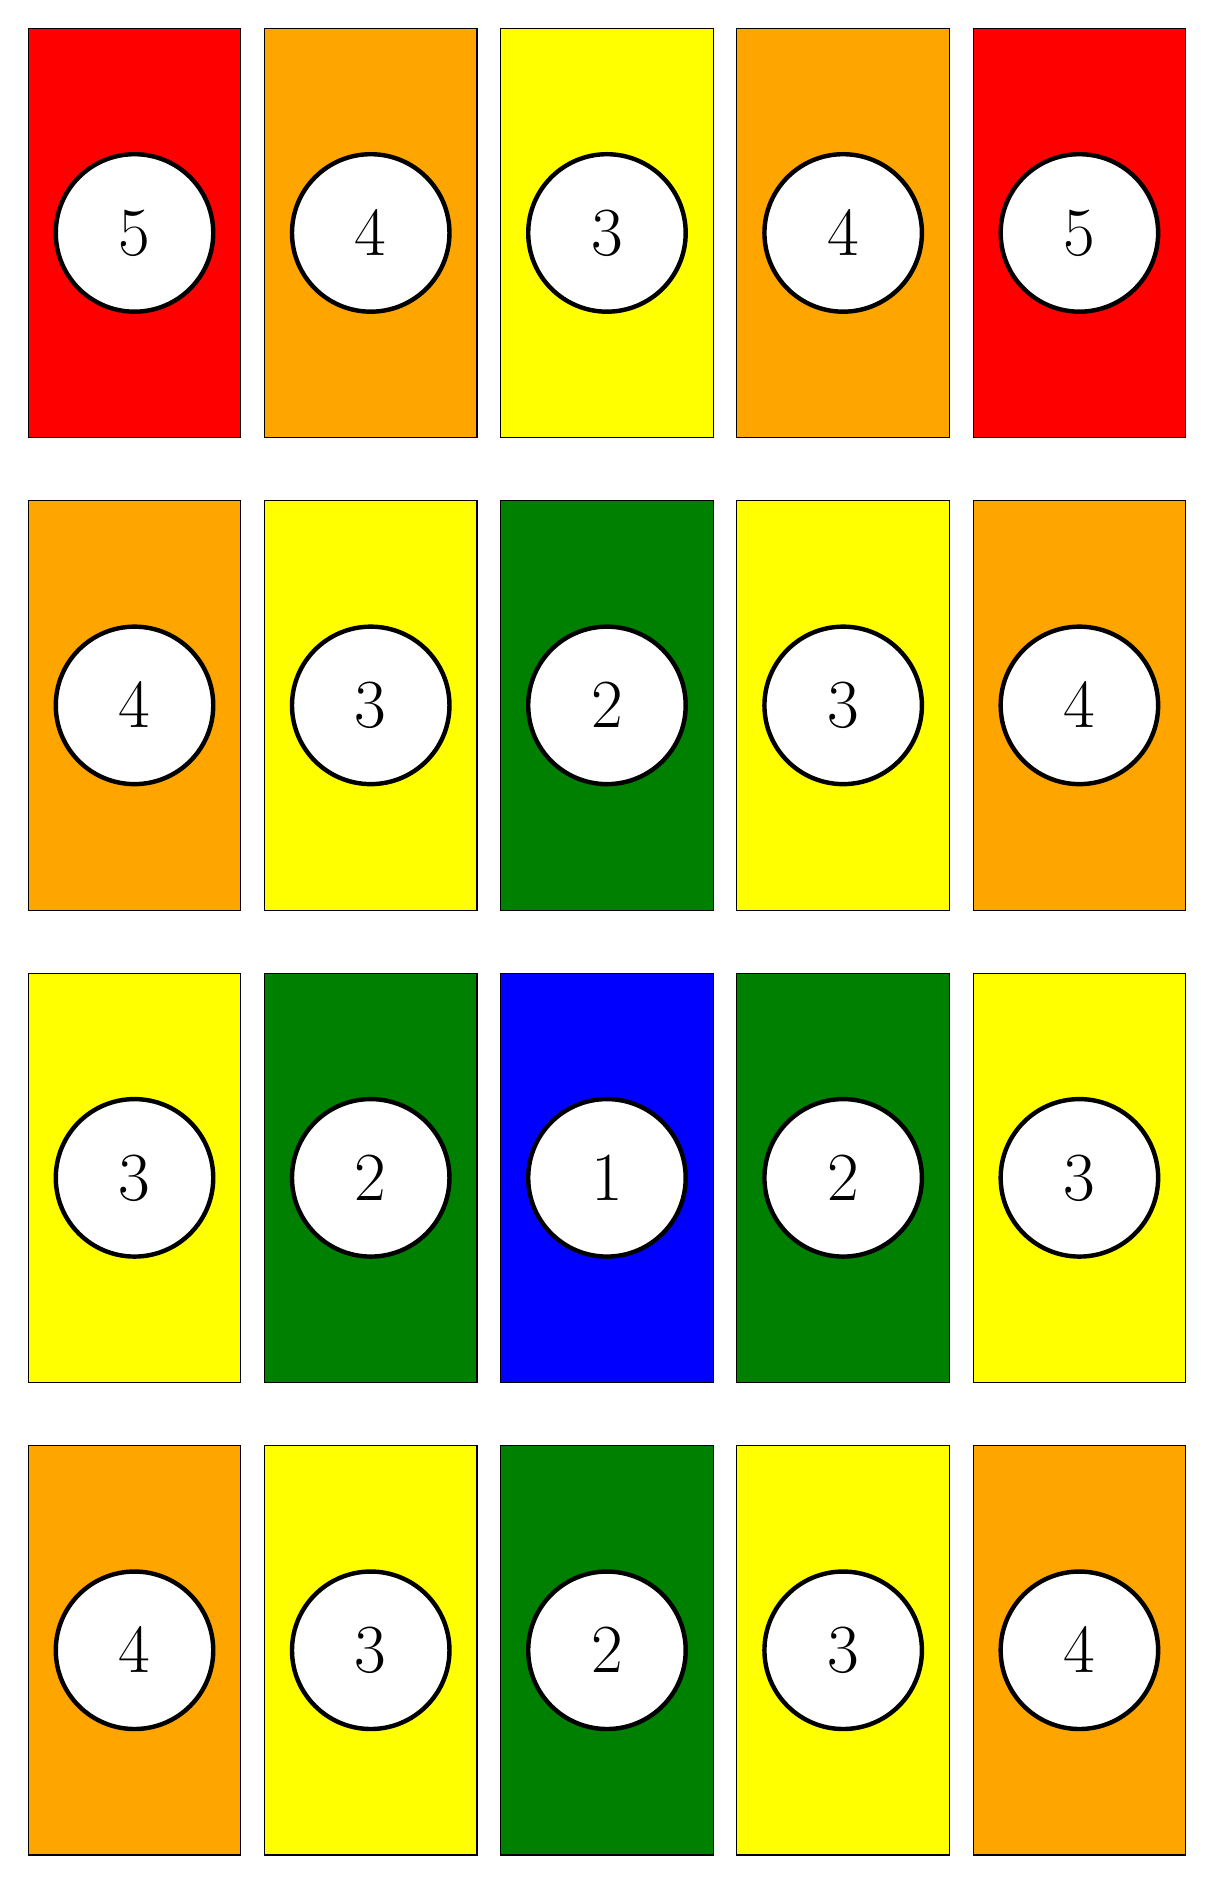
\begin{tikzpicture}
\Huge
%\foreach \i in {-60mm, -30mm, 0mm, 30mm, 60mm}
%	\foreach \j in {-90mm, -30mm, 30mm, 90mm}
%		\node[draw, inner sep=0pt, minimum height=50mm, minimum width=25mm] at (\i,\j) {};
		
\node[score rectangle, fill=Red] at (-60mm,90mm) {};
\node[score circle, fill=White] at (-60mm,90mm) {5};
\node[score rectangle, fill=Orange] at (-30mm,90mm) {};
\node[score circle, fill=White] at (-30mm,90mm) {4};
\node[score rectangle, fill=Yellow] at (0mm,90mm) {};
\node[score circle, fill=White] at (0mm,90mm) {3};
\node[score rectangle, fill=Orange] at (30mm,90mm) {};
\node[score circle, fill=White] at (30mm,90mm) {4};
\node[score rectangle, fill=Red] at (60mm,90mm) {};
\node[score circle, fill=White] at (60mm,90mm) {5};

\node[score rectangle, fill=Orange] at (-60mm,30mm) {};
\node[score circle, fill=White] at (-60mm,30mm) {4};
\node[score rectangle, fill=Yellow] at (-30mm,30mm) {};
\node[score circle, fill=White] at (-30mm,30mm) {3};
\node[score rectangle, fill=Green] at (0mm,30mm) {};
\node[score circle, fill=White] at (0mm,30mm) {2};
\node[score rectangle, fill=Yellow] at (30mm,30mm) {};
\node[score circle, fill=White] at (30mm,30mm) {3};
\node[score rectangle, fill=Orange] at (60mm,30mm) {};
\node[score circle, fill=White] at (60mm,30mm) {4};

\node[score rectangle, fill=Yellow] at (-60mm,-30mm) {};
\node[score circle, fill=White] at (-60mm,-30mm) {3};
\node[score rectangle, fill=Green] at (-30mm,-30mm) {};
\node[score circle, fill=White] at (-30mm,-30mm) {2};
\node[score rectangle, fill=Blue] at (0mm,-30mm) {};
\node[score circle, fill=White] at (0mm,-30mm) {1};
\node[score rectangle, fill=Green] at (30mm,-30mm) {};
\node[score circle, fill=White] at (30mm,-30mm) {2};
\node[score rectangle, fill=Yellow] at (60mm,-30mm) {};
\node[score circle, fill=White] at (60mm,-30mm) {3};

\node[score rectangle, fill=Orange] at (-60mm,-90mm) {};
\node[score circle, fill=White] at (-60mm,-90mm) {4};
\node[score rectangle, fill=Yellow] at (-30mm,-90mm) {};
\node[score circle, fill=White] at (-30mm,-90mm) {3};
\node[score rectangle, fill=Green] at (0mm,-90mm) {};
\node[score circle, fill=White] at (0mm,-90mm) {2};
\node[score rectangle, fill=Yellow] at (30mm,-90mm) {};
\node[score circle, fill=White] at (30mm,-90mm) {3};
\node[score rectangle, fill=Orange] at (60mm,-90mm) {};
\node[score circle, fill=White] at (60mm,-90mm) {4};

\end{tikzpicture}
\end{document}